\documentclass[../../../../main.tex]{subfiles}

\begin{document}

\section*{第1問}

\noindent
[\textbf{解}] $|OA|=x, |OB|=y, |OC|=z$ とする。

\noindent
$\triangle OAB$ に3平方の定理を用いて、
\begin{align}
c^2 &= x^2 + y^2 \tag{1}
\end{align}
同様に
\begin{align}
b^2 &= x^2 + z^2 \tag{2} \\
a^2 &= y^2 + z^2 \tag{3}
\end{align}
したがって
\[
|OP| = \sqrt{x^2+y^2+z^2} = \sqrt{\frac{a^2+b^2+c^2}{2}}
\]
又、(1), (2), (3) を $x, y, z$ についてといて、$(a,b)=(5,3)$ を代入して
\begin{align*}
x &= \sqrt{\frac{-a^2+b^2+c^2}{2}} = \sqrt{\frac{-16+c^2}{2}} \\
y &= \sqrt{\frac{a^2-b^2+c^2}{2}} = \sqrt{\frac{16+c^2}{2}} \\
z &= \sqrt{\frac{a^2+b^2-c^2}{2}} = \sqrt{\frac{34-c^2}{2}}
\end{align*}
これらが存在すれば良いので、
\[
-16+c^2 > 0, \quad 16+c^2 > 0, \quad 34-c^2 > 0
\]
\[
\iff 4 < c < \sqrt{34} \quad (\because c > 0)
\]

\newpage

\section*{第2問}

\noindent
[\textbf{解}] $l$ が $x$ 軸に一致し、$P(0, \sqrt{3}+1)$ となるよう $xy$ 平面をおく。

\begin{center}
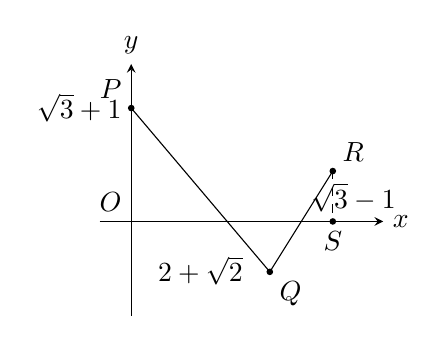
\begin{tikzpicture}[scale=0.8, >=stealth]
  \draw[->] (-0.5,0) -- (4.0,0) node[right] {$x$};
  \draw[->] (0,-1.5) -- (0,2.5) node[above] {$y$};
  \node[above left] at (0,0) {$O$};
  \fill (0,1.8) circle (1.5pt) node[above left] {$P$};
  \node[left] at (0,1.8) {$\sqrt{3}+1$};
  \fill (2.2,-0.8) circle (1.5pt) node[below right] {$Q$};
  \node[below] at (1.1,-0.4) {$2+\sqrt{2}$};
  \fill (3.2,0.8) circle (1.5pt) node[above right] {$R$};
  \node[above right] at (2.7,0.0) {$\sqrt{3}-1$};
  \fill (3.2,0) circle (1.5pt) node[below] {$S$};
  \draw (0,1.8) -- (2.2,-0.8) -- (3.2,0.8);
  \draw[dashed] (3.2,0.8) -- (3.2,0);
\end{tikzpicture}
\end{center}

\noindent
まず、$|PQ| = 2+\sqrt{2}$ より、$Q$ は半径 $2+\sqrt{2}$ の円
\[
x^2 + (y - \sqrt{3} - 1)^2 = (2 + \sqrt{2})^2
\]
上をうごく。同様に
\[
2+\sqrt{2} - (2-\sqrt{2}) \le |PR| \le (2+\sqrt{2}) + (2-\sqrt{2})
\]
\[
2\sqrt{2} \le |PR| \le 4 \quad (\text{間の値もすべてとる})
\]
だから、$R$ は、
\[
8 \le x^2 + (y - \sqrt{3} - 1)^2 \le 16
\]
上をうごく。このうち、$R$ と $x$ 軸との距離が $\sqrt{3}-1$ 以下である部分が求める領域で、右図斜線部（境界含む）。

\begin{center}
\begin{tikzpicture}[scale=0.8, >=stealth]
  % Axes
  \draw[->] (-4.5,0) -- (4.5,0) node[right] {$x$};
  \draw[->] (0,-2.5) -- (0,3.2) node[above] {$y$};
  \node[below left] at (0,0) {$0$};

  % Center P(0, sqrt(3)+1) ~ (0, 2.73)
  \coordinate (P) at (0, 2.732);
  
  % Outer arc R=4, Inner arc R=2*sqrt(2) ~ 2.828
  % Center at y = 2.732.
  % Outer circle passes through (0, -1.268) which is sqrt(3)-3.
  % Line y = sqrt(3)-1 ~ 0.732.
  % Line y = -sqrt(3)+1 ~ -0.732.

  % Shaded region bounded by outer arc, inner arc, y = sqrt(3)-1
  \begin{scope}
    \clip (-4.2, -2.0) rectangle (4.2, 0.732);
    \fill[pattern=north east lines, pattern color=gray] (P) circle (4);
    \fill[white] (P) circle (2.828);
  \end{scope}

  % Draw arcs
  \draw[thick] (P) ++(-60:4) arc (-60:-120:4);
  \draw[thick] (P) ++(-45:2.828) arc (-45:-135:2.828);
  
  % Horizontal boundary line y = sqrt(3)-1
  \draw[dashed] (-4.2, 0.732) -- (4.2, 0.732);
  \node[right] at (4.2, 0.732) {$\sqrt{3}-1$};

  % Labels on y-axis
  \fill (0,2.732) circle (1.5pt) node[left] {$\sqrt{3}+1$};
  \node[right] at (0,0.732) {$\sqrt{3}-1$};
  \node[right] at (0,-0.096) {$\sqrt{3}+1-2\sqrt{2}$};
  \node[right] at (0,-1.268) {$\sqrt{3}-3$};
  \node[left] at (-0.2,-0.732) {$-\sqrt{3}+1$};

  % Labels on x-axis
  \node[below] at (-4,0) {$-4$};
  \node[below] at (-2.828,0) {$-2\sqrt{2}$};
  \node[below] at (2.828,0) {$2\sqrt{2}$};
  \node[below] at (4,0) {$4$};

  % Angle labels
  \node at (-1.5,2.2) {$45^\circ$};
  \node at (1.8,2.5) {$60^\circ$};
  \node at (0.5,1.8) {$30^\circ$};
\end{tikzpicture}
\end{center}

\noindent
この面積 $S$ とする。右下図で、
\begin{align}
S = S_1 - S_2 \tag{1}
\end{align}
となり、
\begin{align*}
S_1 &= 2 \int_{2}^{2\sqrt{3}} \sqrt{16-x^2} \, dx \\
&= 2 \int_{\frac{\pi}{6}}^{\frac{\pi}{3}} 16 \cos^2 \theta \, d\theta \\
&= 16 \left[ \theta + \frac{1}{2} \sin 2\theta \right]_{\pi/6}^{\pi/3} \\
&= \frac{8}{3}\pi
\end{align*}

\begin{center}
\begin{tikzpicture}[scale=0.7, >=stealth]
  % S1 diagram
  \begin{scope}[shift={(0,0)}]
    \draw (-3,0) -- (3,0);
    \draw (0,-1.5) -- (0,0);
    \draw (-2.5,0) arc (-150:-30:2.89);
    \fill[pattern=north east lines, pattern color=gray] (-2.5,0) arc (-150:-30:2.89) -- cycle;
    \node at (0,-0.8) {$S_1$};
    \node[above] at (-2.5,0) {$-2\sqrt{3}$};
    \node[above] at (2.5,0) {$2\sqrt{3}$};
    \node at (0, 0.4) {$30^\circ$};
    \node at (-1.5, 0.4) {$4$};
    \node at (1.5, 0.4) {$4$};
  \end{scope}

  % S2 diagram
  \begin{scope}[shift={(7,0)}]
    \draw (-2.5,0) -- (2.5,0);
    \draw (0,-1.5) -- (0,0);
    \draw (-2,0) arc (-135:-45:2.828);
    \fill[pattern=north east lines, pattern color=gray] (-2,0) arc (-135:-45:2.828) -- cycle;
    \node at (0,-0.8) {$S_2$};
    \node[above] at (-2,0) {$-2\sqrt{2}$};
    \node[above] at (2,0) {$2\sqrt{2}$};
    \node at (1.2, 0.4) {$45^\circ$};
  \end{scope}
\end{tikzpicture}
\end{center}

\begin{align*}
S_2 &= (\text{扇形}) - (\text{三角形}) \\
&= \frac{1}{2} \cdot \frac{\pi}{2} \cdot (2\sqrt{2})^2 - \frac{1}{2} \cdot 2 \cdot 2 \cdot 2 \\
&= 2\pi - 4
\end{align*}
(1)に代入して
\[
S = 4 + \frac{2}{3}\pi
\]

\newpage

\section*{第3問}

\begin{center}
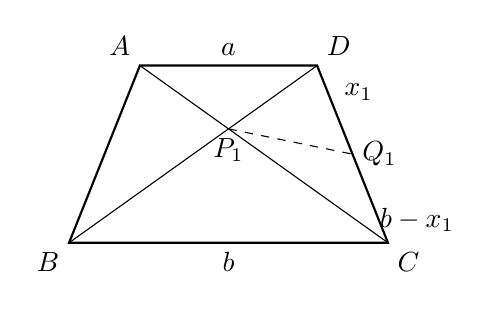
\begin{tikzpicture}[scale=0.9, >=stealth]
  % Top trapezoid diagram
  \coordinate (A) at (1,2.5);
  \coordinate (D) at (3.5,2.5);
  \coordinate (B) at (0,0);
  \coordinate (C) at (4.5,0);
  
  \draw[thick] (A) -- (D) -- (C) -- (B) -- cycle;
  \draw (A) -- (C);
  \draw (B) -- (D);
  
  % Intersection P1
  \coordinate (P1) at (intersection of A--C and B--D);
  \draw[dashed] (P1) -- (4.0, 1.25) coordinate (Q1);

  \node[above left] at (A) {$A$};
  \node[above right] at (D) {$D$};
  \node[below left] at (B) {$B$};
  \node[below right] at (C) {$C$};
  \node[below] at (P1) {$P_1$};
  \node[right] at (Q1) {$Q_1$};

  \node[above] at (2.25,2.5) {$a$};
  \node[below] at (2.25,0) {$b$};
  \node[above right] at (3.75, 1.875) {$x_1$};
  \node[below right] at (4.25, 0.625) {$b-x_1$};
\end{tikzpicture}

\vspace{0.5cm}

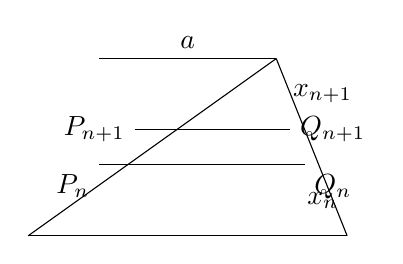
\begin{tikzpicture}[scale=0.9, >=stealth]
  % General step diagram
  \coordinate (A) at (1,2.5);
  \coordinate (D) at (3.5,2.5);
  \coordinate (B) at (0,0);
  \coordinate (C) at (4.5,0);

  \draw (A) -- (D);
  \draw (B) -- (C);
  \draw (B) -- (D);
  \draw (C) -- (D);

  \draw (1.5, 1.5) node[left] {$P_{n+1}$} -- (3.7, 1.5) node[right] {$Q_{n+1}$};
  \draw (1.0, 1.0) node[below left] {$P_n$} -- (3.9, 1.0) node[below right] {$Q_n$};

  \node[above] at (2.25,2.5) {$a$};
  \node[right] at (3.6, 2.0) {$x_{n+1}$};
  \node[right] at (3.8, 0.5) {$x_n$};
\end{tikzpicture}
\end{center}

\noindent
[\textbf{解}] (1) $B=P_0, C=Q_0$ とする。$\triangle P_n Q_n D$, $\triangle AD Q_n$ に注目し、相似から
\[
x_{n+1} : x_n - x_{n+1} = a - x_{n+1} : x_{n+1}
\]
\[
\therefore x_{n+1} = \frac{a x_n}{a + x_n} \tag{1}
\]
$x_n \neq 0$ だから、$y_n = \frac{1}{x_n}$ として、(1)の両辺逆数をとって、
\[
y_{n+1} = y_n + \frac{1}{a}
\]
$y_0 = \frac{1}{x_0} = \frac{1}{b}$ だから、くり返し用いて、
\[
y_n = \frac{n}{a} + \frac{1}{b}
\]
\[
\therefore x_n = \frac{1}{\frac{n}{a} + \frac{1}{b}} = \frac{ab}{a + bn}
\]

\noindent
(2) 辺 $P_{n+1} Q_{n+1}$ を底辺とみたときの $\triangle D P_{n+1} Q_n$ の高さ $h_n$ は
\[
h_n = \frac{H}{b} x_n \quad (n \ge 1)
\]
だから
\begin{align*}
F_n &= \frac{1}{2} h_n x_{n+1} = \frac{H}{2b} \cdot \frac{ab}{a+bn} \cdot \frac{ab}{a+b(n+1)} \\
&= \left( \frac{1}{a+bn} - \frac{1}{a+b(n+1)} \right) \frac{a^2 H}{2}
\end{align*}
となり、
\[
\sum_{k=1}^n F_k = \frac{a^2 H}{2} \left( \frac{1}{a+b} - \frac{1}{a+b(n+1)} \right) \xrightarrow{n \to \infty} \frac{H a^2}{2(a+b)}
\]

\newpage

\section*{第4問}

\noindent
[\textbf{解}] $|AP| = x \ (0 < x < a)$ とおく。
\[
|PQ| = x, \quad |PP'| = a-x
\]
だから、三角柱の体積 $V(x)$ として
\begin{align*}
V(x) &= \frac{\sqrt{3}}{4} |PQ|^2 |PP'| \quad (\because \triangle PQR \text{は正三角形}) \\
&= \frac{\sqrt{3}}{4} x^2 (a-x)
\end{align*}
と書ける。$x, a-x > 0$ から AM-GM より
\[
V(x) \le \frac{\sqrt{3}}{27} a^3 \equiv V_0 \quad \left(\text{等号成立は } \frac{1}{2}x = a-x \text{ つまり } x = \frac{2}{3}a \text{ の時}\right)
\]
したがって、もとめるのは $x = \frac{2}{3}a$ である。（以上(1)）

\noindent
$\bar{V} = \frac{\sqrt{3}}{12} a^3$
だから
\[
\frac{V_0}{\bar{V}} = \frac{\frac{\sqrt{3}}{27} a^3}{\frac{\sqrt{3}}{12} a^3} = \frac{4}{9}
\]

\newpage

\section*{第5問}

\noindent
[\textbf{解}] まず、一辺の長さを2として考える。この時 $A(1,0), B(0,-1), C(-1,0), D(0,1)$ となるよう座標を定める。$Q$ の $y$ 座標を $t \ (0 \le t \le 1)$ とする。

\begin{center}
\begin{tikzpicture}[scale=1.2, >=stealth]
  % Axes
  \draw[->] (-1.8,0) -- (1.8,0) node[right] {$x$};
  \draw[->] (0,-1.5) -- (0,1.5) node[above] {$y$};
  
  % Rhombus ABCD
  \coordinate (A) at (1,0);
  \coordinate (B) at (0,-1);
  \coordinate (C) at (-1,0);
  \coordinate (D) at (0,1);
  
  \draw[thick] (A) -- (D) -- (C) -- (B) -- cycle;
  
  \node[right] at (A) {$A$};
  \node[below] at (B) {$B$};
  \node[left] at (C) {$C$};
  \node[above right] at (D) {$D$};

  \node[left] at (-1,0) {$-1$};
  \node[below left] at (0,-1) {$-1$};

  % Points Q, P, R, T
  \coordinate (Q) at (0.6, 0.4);
  \coordinate (P) at (-0.4, 0.4);
  \coordinate (R) at (-0.4, -0.6);
  \coordinate (T) at (-0.4, 0);

  % Region ABRPQ
  \fill[pattern=north east lines, pattern color=gray] (A) -- (Q) -- (P) -- (R) -- (B) -- cycle;
  \draw[thick] (Q) -- (P) -- (R);

  \node[above right] at (Q) {$Q$};
  \node[above left] at (P) {$P$};
  \node[below left] at (R) {$R$};
  \node[above left] at (T) {$T$};
  \node[right] at (0, 0.4) {$t$};
  \node[right] at (0, 0.8) {$1-t$};

  \draw[dashed] (P) -- (0.6, 0.4);
\end{tikzpicture}
\hspace{1cm}
\begin{tikzpicture}[scale=1.2, >=stealth]
  % Curve in st-plane
  \draw[->] (-1.5,0) -- (0.5,0) node[right] {$x$};
  \draw[->] (0,-0.5) -- (0,1.5) node[above] {$y$};
  \node[below left] at (0,0) {$0$};

  \draw[thick, domain=0:1, samples=50] plot ({- (sqrt(\x) - 1)^2}, \x);
  \draw[dashed] (-1,0) -- (0,1) node[midway, above right] {$x+y=1$};

  \begin{scope}
    \clip (-1.5, 0) rectangle (0, 1);
    \fill[pattern=horizontal lines, pattern color=gray, domain=0:1, samples=50] 
      plot ({- (sqrt(\x) - 1)^2}, \x) -- (-1,0) -- cycle;
  \end{scope}

  \node[left] at (-1,0) {$-1$};
  \node[left] at (P) {$P$};
  \node[below] at (1,0) {$1$};
\end{tikzpicture}
\end{center}

\noindent
この時 $P(s,t) \ (-1+t \le s \le 1-t)$ とおける。

\noindent
ただし、$0 < s$ の時、明らかに折れ線 $TPU$ は $ABCD$ の面積を2等分しないので、$-1+t \le s \le 0$ として良い。この時、$PU$ と辺 $BC$ の交点 $R$ として $R(s, -1-s)$

\noindent
だから、五角形 $ABRPQ$ の面積が $ABCD$ の面積の $\frac{1}{2}$ に等しい時、$PR$ と $x$ 軸の交点 $T$ として
\[
\triangle CRT = \Box AQPT
\]
\[
\therefore \frac{1}{2}(1+s)^2 = \frac{1}{2} t \{ (1-t-s) + (1-s) \} = \frac{1}{2} t (2 - 2s - t)
\]
\[
\therefore s^2 + 2s + 1 = 2t - 2st - t^2
\]
\begin{align}
\therefore s^2 + t^2 + 2st + 2s - 2t + 1 = 0 \tag{1}
\end{align}
これは放物線を表し、$P$ の概形は右図のゆえ、斜線部の面積をもとめれば良い。(1)を $s$ についてとくと
\begin{align*}
s &= -(t+1) \pm \sqrt{(t+1)^2 - (t-1)^2} \\
&= -(t+1) \pm 2\sqrt{t} \quad (\because t \ge 0)
\end{align*}
$t=0$ で $s=0$ より、複号正を採用して
\[
s = -(\sqrt{t} - 1)^2
\]
だから、もとめる面積 $V$ は
\begin{align*}
V &= \int_0^1 (1 - t + (\sqrt{t}-1)^2) \, dt \\
&= \int_0^1 2(1-\sqrt{t}) \, dt \\
&= 2 \left[ t - \frac{2}{3} t^{3/2} \right]_0^1 = \frac{2}{3}
\end{align*}
となる。一辺 $a$ のとすると、これの $\frac{a^2}{2}$ 倍ゆえ
\[
V = \frac{1}{3} a^2
\]
となる。

\newpage

\section*{第6問}

\noindent
[\textbf{解}] $O(0,0), A(1,1), B(2, 2^n)$ となる。

\noindent
$f(x) = ax^2 + bx \ (a \neq 0)$ とおける。($\because f(0)=0$) $A,B$ の座標を代入して
\[
\begin{cases} a+b=1 \\ 4a+2b=2^n \end{cases} \iff \begin{cases} a = 2^{n-1}-1 \\ b = 2 - 2^{n-1} \end{cases} \tag{1}
\]
となる。ここで、$g_n(x) = x^n - f(x)$ とおくと、(1)より
\begin{align*}
g_n(x) &= x \left\{ x^{n-1} - ax - b \right\} \\
&= x \left[ (2^{n-1}-1)(1-x) - (1-x^{n-1}) \right] \\
&= x(1-x) \left[ 2^{n-1} - 1 - (x^{n-2} + \dots + x + 1) \right] \tag{2}
\end{align*}
である。$0 \le x \le 2$ の時、($n \in \mathbb{Z}_{\ge 3}$ から)
\[
1 + x + \dots + x^{n-2} \le 1 + 2 + \dots + 2^{n-2} = 2^{n-1}-1
\]
だから、
\[
2^{n-1}-1 - (1 + \dots + x^{n-2}) \ge 0
\]
なので、(2)より
\[
\begin{cases} 0 \le x \le 1 \text{ の時 } g_n(x) \ge 0 \\ 1 \le x \le 2 \text{ の時 } g_n(x) \le 0 \end{cases}
\]
である。したがって、
\[
S_1 = \int_0^1 g_n(x) \, dx, \quad S_2 = -\int_1^2 g_n(x) \, dx
\]
だから、
\begin{align*}
S_1 = S_2 &\iff \int_0^2 g_n(x) \, dx = 0 \\
&\iff \left( \frac{1}{n+1} - \frac{1}{6} \right) 2^{n+1} = \frac{4}{3}
\end{align*}
をみたす $n$ をもとめれば良い。$n \ge 5$ の時、左辺は0以下になり不適だから、$n \ge 3$ とあわせて $n=3,4$ をしらべれば良い。
\[
\begin{cases} n=3 \text{ の時、(左辺)} = \left(\frac{1}{4}-\frac{1}{6}\right) 2^4 = \frac{4}{3} \\ n=4 \text{ の時、(左辺)} = \left(\frac{1}{5}-\frac{1}{6}\right) 2^5 = \frac{16}{15} \end{cases}
\]
より、$n=3$ のみ適する。以上から、もとめるのは $n=3$ である。

\end{document}
